\chapter{Prezentarea contribuțiilor autorului}
\label{cap:contributii}
În acest capitol se face prezentarea contribuțiilor autorului: un studiu comparativ a metodelor existente de detecția obiectelor și segmentarea semantică a imaginilor bazate pe rețele neuronale convoluționale.\newline
Se vor analiza în detaliu algoritmii care au la bază inteligență artificială deorece performanța acestora în domeniul prelucrării imaginilor depășește semnificativ orice altă metodă (algoritmi de nivel mai jos, cum ar fi algoritmii de thresholding) datorită faptului că rețelele neuronale nu sunt influențate de zgomotul din imagini, dar și pentru că sunt capabile de a produce rezultate în timp real \cite{cat_amz}.


\section{Categorii de algoritmi de segmentarea imaginilor}
Segmentarea imaginilor este unul dintre cele mai importante procese în domeniul viziunii artificiale moderne. Segmentarea imaginilor înseamnă etichetarea fiecărui pixel, ca aparținând unui obiect din imagine. Segmentele rezultate corespund unităților structurale (obiecte) din scenă. Segmentarea imaginilor este o problemă dificilă, pentru că nu există un model matematic care ar putea descrie bine procesul \cite{cat_amz}.\newline
Există un număr mare de algoritmi propuse în literatură, care vor fi prezentate în acest capitol. Favorizarea unei metode depinde numai de situație și de tipul de imagine care trebuie segmentat. Nu există nicio metodă universală, care produce rezultate bune pe fiecare tip de imagine. Chiar și alegerea metodei corespunzătoare pentru un tip de imagine este o problemă dificilă. Metode dezvoltate pentru un tip de imagine pot produce rezultate proaste pe alt tip de imagine.\newline
Technicile de segmentare pot fi plasate în trei clase mai mari:
\begin{itemize}
	\item algoritmi clasici bazate pe matematică sau metode statistice
	\item technici bazate pe inteligență artificială
	\item alte technici care fie sunt metode hibride, fie nu moștenesc din nicio categorie
\end{itemize}

Algoritmii clasici includ detecția marginilor obiectelor(\textit{edge/boundary detection)}, methode de thresholding (\textit{characteristic histogram thresholding)}, extragerea regiunilor (\textit{region extraction/region growing)} și abordări semantice și sintactice.\newline
Metodele de segmentare din domeniul inteligenței artificiale sunt de regulă metode care folosesc rețele neuronale.\newline

\subsection{Technici Bazate pe Rețele Neuronale Artificiale}
Începând cu anii 1990, rețelele neuronale au apărut și în domeniul prelucrării imaginilor și a viziunii artificiale. Având capabilități dorite (e.g. sunt insensibile la zgomotul din imagini, pot funcționa în timp real) au devenit foarte populare. Bineînțeles, diferite rețele neuronale au fost aplicate cu diferite nivele de succes; rețelele feed-forward back-propagation s-au dovedit a fi cele mai efective.\newline
Rețelele neuronale capabile de segmentare semantică pot fi împărțite în două categorii: rețele supravegheate și rețele nesupravegheate. Rețelele supravegheate au nevoie de set de antrenare etichetată, adică imagini pe care regiunile de interes sunt notate, având la îndemână și tipul obiectelor din zonele respective. Metodele nesupravegheate (numite și \textit{clustering processes}) sunt semi- sau total automate.

\subsubsection{Rețele supravegheate}
Rețelele neuronale care sunt antrenare cu învățare supravegheată au nevoie de un operator uman pentru a alege imaginile de antrenare și pentru a le segmenta în \textit{k} regiuni, fiecare fiind etichetat (cu tipul obiectului în regiune). Architectura propusă este antrenată folosind imaginile etichetate ca set de antrenare. După antrenare, rețeaua neuronală va fi capabilă de a segmenta imagini similare, asignând etichete pentru regiuni folosind cunoștințele acumulate la faza de antrenare.

\subsection{Detecția și Localizarea Obiectelor}
Este o confuzie generală între clasificarea imaginilor și detecția obiectelor din scene. Clasificarea imaginilor (\textit{image classification}) constă în obținerea unei predicții la ieșirea unui sistem referitor la tipul de obiect care era plasat în imaginea de intrare. Pe de altă parte, dacă vrem să identificăm locația obiectelor într-o imagine, și de exemplu să le numărăm numărul instanțelor unui obiect, putem folosi algoritmi de detecția obiectelor (\textit{object detection and localization}).\newline
Eficiența unui algoritm de localizare se măsoară folosind un algoritm de \textit{Intersect over Union}; când măsurăm performanța rețelei antrenate, la stratul de intrare dăm imagini conținând obiecte care pot fi recunoscute și localizate de rețea, acesta specificând la stratul de ieșire predicția coordonatelor bounding-boxului fiecărui obiect. Aceste coordonate se compară cu cele reale, și se calculează Intersect over Union între dreptunghiurile definite de coordonatele specificate de rețea și dreptunghiurile reale (imaginile fiind etichetate avem la îndemână dreptunghiurile care conțin cu adevărat obiectele din imagini).
%object detection and localization
\begin{figure}[h!]
    	\centering
	\captionsetup{justification=centering, margin=2cm}
	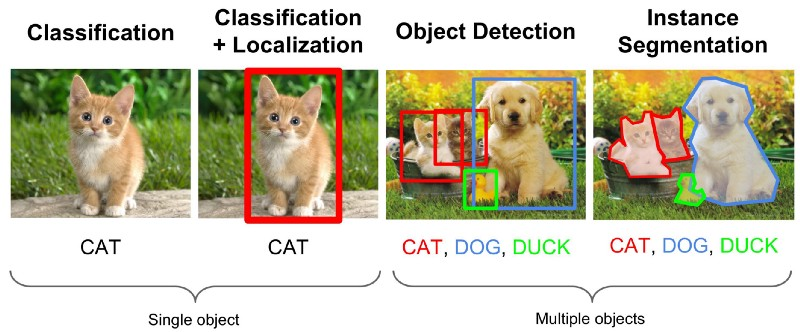
\includegraphics[width=0.9\textwidth]{figures/class_detect_segment.jpeg}
	\caption{Detecția obiectelor \cite{class_detect_segment}}
	\label{fig:class_detect_segment}
\end{figure}

\url{https://leonardoaraujosantos.gitbooks.io/artificial-inteligence/content/object_localization_and_detection.html}
\url{https://medium.com/nanonets/how-to-do-image-segmentation-using-deep-learning-c673cc5862ef}
Cinci abordări pentru detecția și localizarea obiectelor vor fi analizate și comparate:
\begin{itemize}
	\item RCNN
	\item Fast RCNN
	\item Faster RCNN
	\item Yolo
	\item SSD
\end{itemize}

\subsubsection{RCNN}
\url{https://towardsdatascience.com/r-cnn-fast-r-cnn-faster-r-cnn-yolo-object-detection-algorithms-36d53571365e}
Când se face detectarea obiectelor o problemă cu care ne întâlnim inevitabil este faptul că în majoritatea cazurilor nu o să fie numai un bounding box pentru o scenă pentru că imaginea respectivă poate să conțină numeroase obiecte de interes și nu putem să știm dinainte câte. Din acest motiv nu putem să folosim o rețea neuronală standard extinsă cu un strat fully connected.\newline
RCNN (Regions + CNN) este o metodă care se bazează pe o metodă externă de propunere de regiuni care găsește regiunile de interes, și le găsește repede. Algoritmul extern de propunere de regiuni se numește \textit{selective search}.\newline
Chiar și accelerând pasul de generare de regiuni de interes, problema cu RCNN este că nu este destul de rapid.\newline
Cu ajutorul selective search se generează 2000 de regiuni cu potențial mare de a conține vreun obiect de interes. Regiunile generate de selective search sunt numite propuneri de regiuni (\textit{region proposals}). Aceste propuneri de regiuni sunt introduse într-o rețea convoluțională care produce un vector de trăsături. Astfel rețeaua convoluțională funcționează ca un extractor de trăsături, iar stratul de ieșire conține trăsăturile extrase care sunt introduse într-un support vector machine pentru a clasifica prezența unui obiect în propunerea de regiune.\newline
RCNN are și câteva dezavantaje:
\begin{itemize}
	\item chiar și cu accelerarea pasului de propunere de regiuni timpul de antrenare a rețelei este lung, pentru că pentru fiecare imagine este nevoie de clasificarea a 2000 de propuneri de regiuni
	\item nu poate funcționa în timp real, pentru că detectarea obiectelor durează 47 de secunde în medie pentru imagine
	\item algoritmul selective search nu poate fi îmbunătățit, nici nu poate să învețe. Asta poate duce la generarea neadecvată a propunerilor de regiuni.
\end{itemize}

\subsubsection{Fast RCNN}
\url{https://towardsdatascience.com/r-cnn-fast-r-cnn-faster-r-cnn-yolo-object-detection-algorithms-36d53571365e}
Autorii articolului de RCNN au rezolvat câteva din problemele modelului RCNN pentru a construi un algoritm mai rapid pentru detectarea obiectelor. Acest algoritm îmbunătăți se numește Fast RCNN și este similar cu RCNN. Însă în loc de introducerea propunerilor de regiuni într-un CNN, se introduc imaginile în CNN pentru a genera o hartă de trăsături extrase cu o rețea convoluțională. Din această mapă identificăm propunerile de regiuni și folosim un strat softmax pentru a produce predicții de clasificare pentru regiuni.\newline
Fast RCNN este mai rapid decât predecesorul lui pentru că nu trebuie să introducem 2000 propuneri de regiuni în rețeaua convoluțională de fiecare dată; în schimb operația de convoluție se face o dată per imagine, pentru a genera harta trăsăturilor convoluționale.

%RCNN vs Fast RCNN training and testing times
\begin{figure}[h!]
    	\centering
	\captionsetup{justification=centering, margin=2cm}
	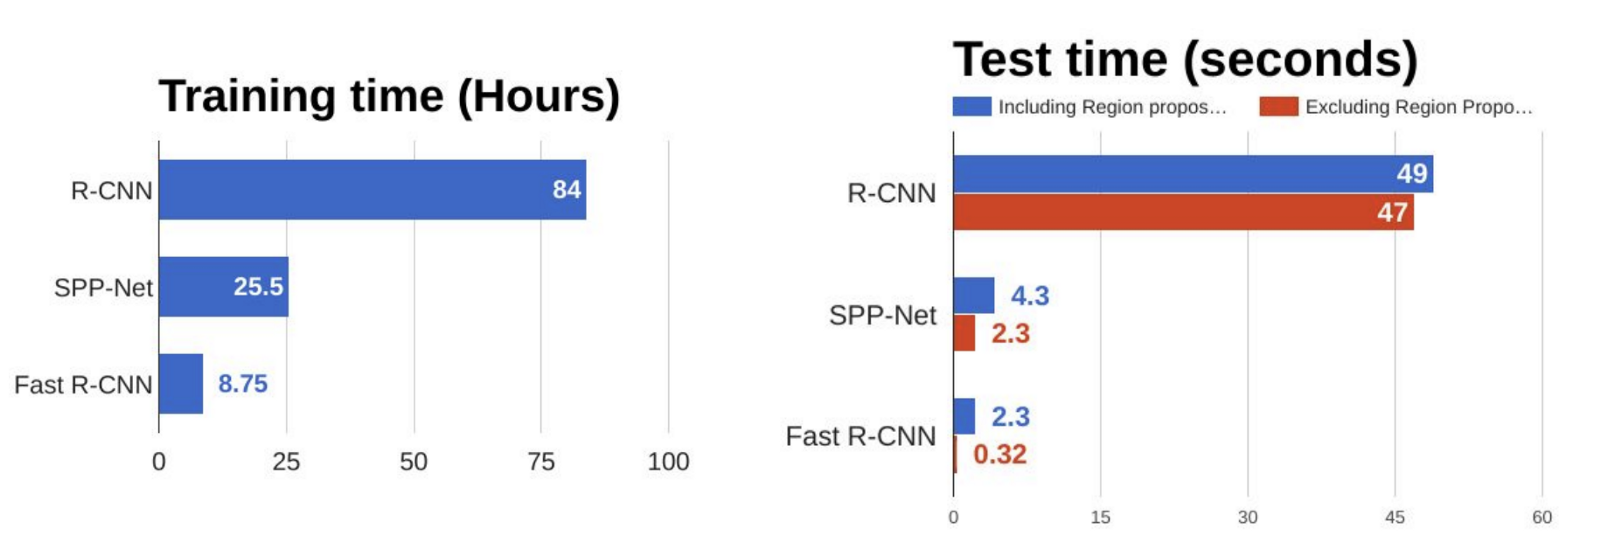
\includegraphics[width=0.9\textwidth]{figures/rcnn_vs_fast_rcnn_time.png}
	\caption{Diferența semnificativă dintre timpul de antrenare și testare între RCNN și Fast RCNN \cite{rcnn_vs_fast_rcnn}}
	\label{fig:class_detect_segment}
\end{figure}
Din acest grafic putem vedea că diferența dintre vitezele a rețelelor este semnificativă. Când ne uităm la performanța rețelei Fast RCNN observăm că performanța lui este mult mai bună fără folosirea metodei de propunere de regiuni. Deci algoritmul de propunere de regiuni este un bottleneck pentru Fast RCNN, afectând semnificativ performanța.

\subsubsection{Faster RCNN}
Ambii algoritmi de mai sus (RCNN și Fast RCNN) folosesc algoritmul selective search pentru a găsi propuneri de regiuni - regiuni cu potențial mare de a conține vreun obiect de interes. Acest algoritm este unul lent, consumă mult timp deci afectează performanța rețelei.\newline
Faster RCNN este similar cu Fast RCNN privind că și aici din imaginea introdusă se generează o hartă de trăsături convoluționale. În schimb aici nu se folosește selective search pentru a găsi regiunile de interes în harta de trăsături; în loc de acesta, o rețea separată este antrenată pentru a găsi predicții pentru coordonaterle regiunilor de interes. Regiunile previzionate sunt remodelate cu un strat RoI pooling și rezultatul este clasificat.

%RCNN vs Fast RCNN vs Faster RCNN testing time
\begin{figure}[h!]
    	\centering
	\captionsetup{justification=centering, margin=2cm}
	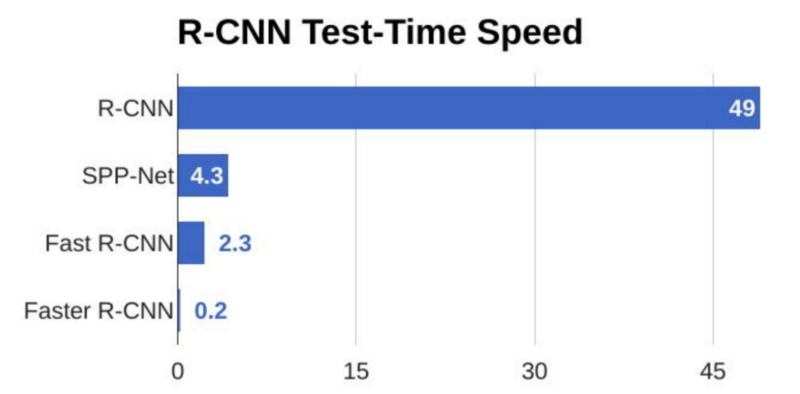
\includegraphics[width=0.8\textwidth]{figures/faster_rcnn_speed.png}
	\caption{Diferența dintre timpul de testare între  Fast RCNN și  Faster RCNN \cite{rcnn_vs_fast_rcnn}}
	\label{fig:class_detect_segment}
\end{figure}
Se vede că Faster RCNN este mult mai rapid decât predecesorii săi. Deja se poate folosi și pentru detectare de obiecte în timp real.

\subsubsection{YOLO - You Only Look Once}
Până aici fiecare algoritm folosește regini pentru a localiza obiectele de interes în imagine. În loc să se uită la imaginea întreagă, rețeaua încearcă să găsească obiecte în părți care au potențial mare de a conține vreun obiect de interes.\newline
YOLO sau You Only Look Once este un algoritm de detectare de obiecte foarte diferit de algoritmii pe care le-am văzut până acum, fiindcă o singură rețea convoluțională este folosit atât pentru predicția bounding boxurilor cât și pentru clasificarea obiectelor din acestea.

%YOLO functioning #1
\begin{figure}[h!]
    	\centering
	\captionsetup{justification=centering, margin=2cm}
	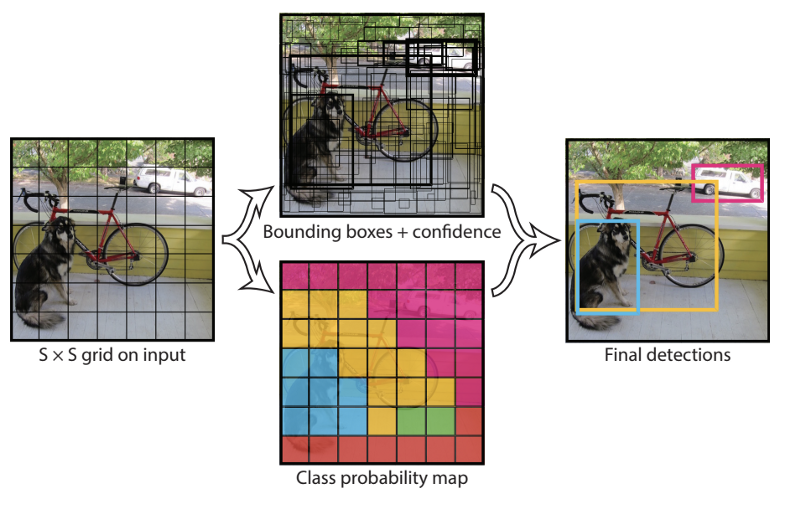
\includegraphics[width=0.8\textwidth]{figures/yolo1.png}
	\caption{YOLO \cite{rcnn_vs_fast_rcnn}}
	\label{fig:class_detect_segment}
\end{figure}
YOLO ia imaginea întreagă, o împarte într-o matrice de SxS, și în fiecare celulă a matricei ia $m$ bounding boxuri. Pentru fiecare rețeua calculează o probabilitățile de a conține diferitele obiectele de interes. Regiunile care au probabilitatea de a conține vreun obiect este peste un anumit prag sunt alese și folosite pentru localizarea obiectului în imagine.\newline
YOLO este mult mai rapid (45 de cadre pe secundă) decât alte algoritmi de detectare de obiecte dezavantajul lui fiind obiectele mici din imagine.






Titlul acestui capitol nu este unul impus și nici nu corespunde neapărat unui singur capitol. Titlul indică mai degrabă o parte (importantă și centrală, de altfel) a lucrării, în care se prezintă ceea ce s-a realizat efectiv: contribuțiile autorului. Organizarea acestei părți este dependentă și specifică fiecărei lucrări în parte și este stabilită de către fiecare autor după cum i se pare mai potrivit pentru tema lui. Ea poate cuprinde prezentarea unor concepte teoretice (unelte sau tehnici matematice folosite în lucrare, prezentarea sau introducerea unor concepte teoretice etc.), o analiză a diferitelor metode/algoritmi/tehnologii etc. luate în considerare sau dezvoltate de către autor, o prezentare a unui design (mai mult sau mai puțin detaliat) sau chiar detalii a unei eventuale implementări/prototip, dacă e cazul.

Trebuie remarcat însă faptul că această parte reprezintă contribuția personală a autorului, chiar dacă ea constă de exemplu doar dintr-o analiză comparativă a unor metode/algoritmi, și în nici un caz ea nu poate fi sinteza unor texte preluate din alte surse. Prin urmare, orice informații sunt prezentate aici, ele trebuie să corespundă cel puțin unei interpretări/analize critice personale a autorului, dacă nu chiar unor idei originale ale acestuia. 

\subsection{Dimensiune}

Împreună cu capitolul (partea) următor reprezintă cca. 70\% din lucrare. 


\section{Examples: lists, figures, tables, equations}

Așa arată o listă de elemente nenumerotate:
\begin{itemize}
  \item element 1
  \item element 2
  \item \dots
\end{itemize}


Așa arată o listă de elemente numerotare:
\begin{itemize}
  \item element 1
  \item element 2
  \item \dots
\end{itemize}


Așa arată o listă în text: 
\begin{inparaenum}[(\itshape 1 \upshape)]
  \item element 1, 
  \item element 2, 
  \item \dots
\end{inparaenum}

\textbf{Atenție}: orice tabel, figura sau ecuație (formulă) trebuie referite \textit{explicit} în text explicit (de genul: în Figura X este ulustrat \dots, în Tabelul Y se poate vedea \dots), pentru că Latex le poate plasa chiar și pe altă pagină decât acolo unde vrem noi să ne referim la ele. Vedeți exemple de mai jos!

Tabelul~\ref{table:example} ilustrează un exemplu de tabel. Un editor on-line de tabele poate fi găsit la \url{http://www.tablesgenerator.com/}. 

\begin{table}[t]
\centering                          % tabel centrat 
\begin{tabular}{|c|c|c|c|}          % 4 coloane centrate 
\hline\hline                        % linie orizontala dubla
Case & Method\#1 & Method\#2 & Method\#3 \\ [0.5ex]   % inserare tabel
%heading
\hline                              % linie orizontal simpla
1 & 50 & 837 & 970 \\               % corpul tabelului 
2 & 47 & 877 & 230 \\
3 & 31 & 25 & 415 \\[1ex]           % [1ex] adds vertical space
\hline                              
\end{tabular}
\caption{Nonlinear Model Results}   % titlul tabelului
\label{table:example}                % \label{table:nonlin} introduce eticheta folosita pentru referirea tabelului in text; referirea in text se va face cu \ref{table:nonlin}
\end{table}

În Figura~\ref{fig:exemplu} 

\begin{figure}
    \centering
    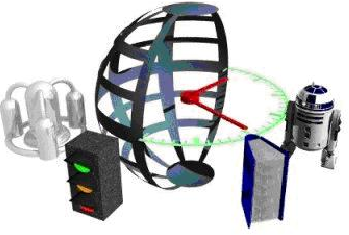
\includegraphics[width=0.5\textwidth]{image}
    \caption{Numele figurii}
    \label{fig:exemplu}
\end{figure}


Formula~(\ref{eq:example}) arată modul de calcul al lui $\Delta$:
\begin{equation} \label{eq:example}
    \Delta =\sum_{i=1}^N w_i (x_i - \bar{x})^2 .
\end{equation}


Algoritmul~\ref{alg:example} este un exemplu de descriere pseudo-cod a unui algoritm, preluat de la \href{http://en.wikibooks.org/wiki/LaTeX/Algorithms#Typesetting_using_the_algorithm2e_package}{http://en.wikibooks.org/wiki/LaTeX}. El utilizează pachetul \textit{algorithm2e}. Alternativ, puteți utiliza pachetele \textit{algorithmic} sau \textit{program}. 

\begin{algorithm}
 \KwData{this text}
 \KwResult{how to write algorithm with \LaTeX2e }
 initialization\;
 \While{not at end of this document}{
  read current\;
  \eIf{understand}{
   go to next section\;
   current section becomes this one\;
   }{
   go back to the beginning of current section\;
  }
 }
 \caption{How to write algorithms}
 \label{alg:example}
\end{algorithm}
